% Side-by-side vertical RND pipelines for Section 9. Compile: latexmk -pdf rnd_pipeline_comparison.tex
%
% Two pipelines, one per column, read TOP TO BOTTOM: CleanRL's PPO + RND on the left, this
% project's SAC + RND (the run-5 original-small stack, the RND of Table 66) on the right. The two
% columns are row-aligned, so a horizontal line across the page compares the same pipeline stage in
% the two implementations.
%
% Deliberately vertical, and deliberately drawn at the document's own text width (5.5 in) so it is
% included at scale 1.0. Figure 16 is horizontal and 11.08 in wide, so at width=\linewidth it is
% scaled to about 0.50 and its \small node text prints at roughly 4.5 pt — half the body font. Every
% text here is at least 10 pt at print scale, per the draw-or-diagrams rule.
%
% Fill encodes the comparison, not the role:
%   white  — the stage is the same in both implementations
%   orange — the stage differs, and the difference is written into the box
\documentclass[tikz,border=4pt]{standalone}
\usepackage{amsmath}
\usepackage{amssymb}
\usetikzlibrary{arrows.meta,positioning,fit,backgrounds,calc}

\begin{document}
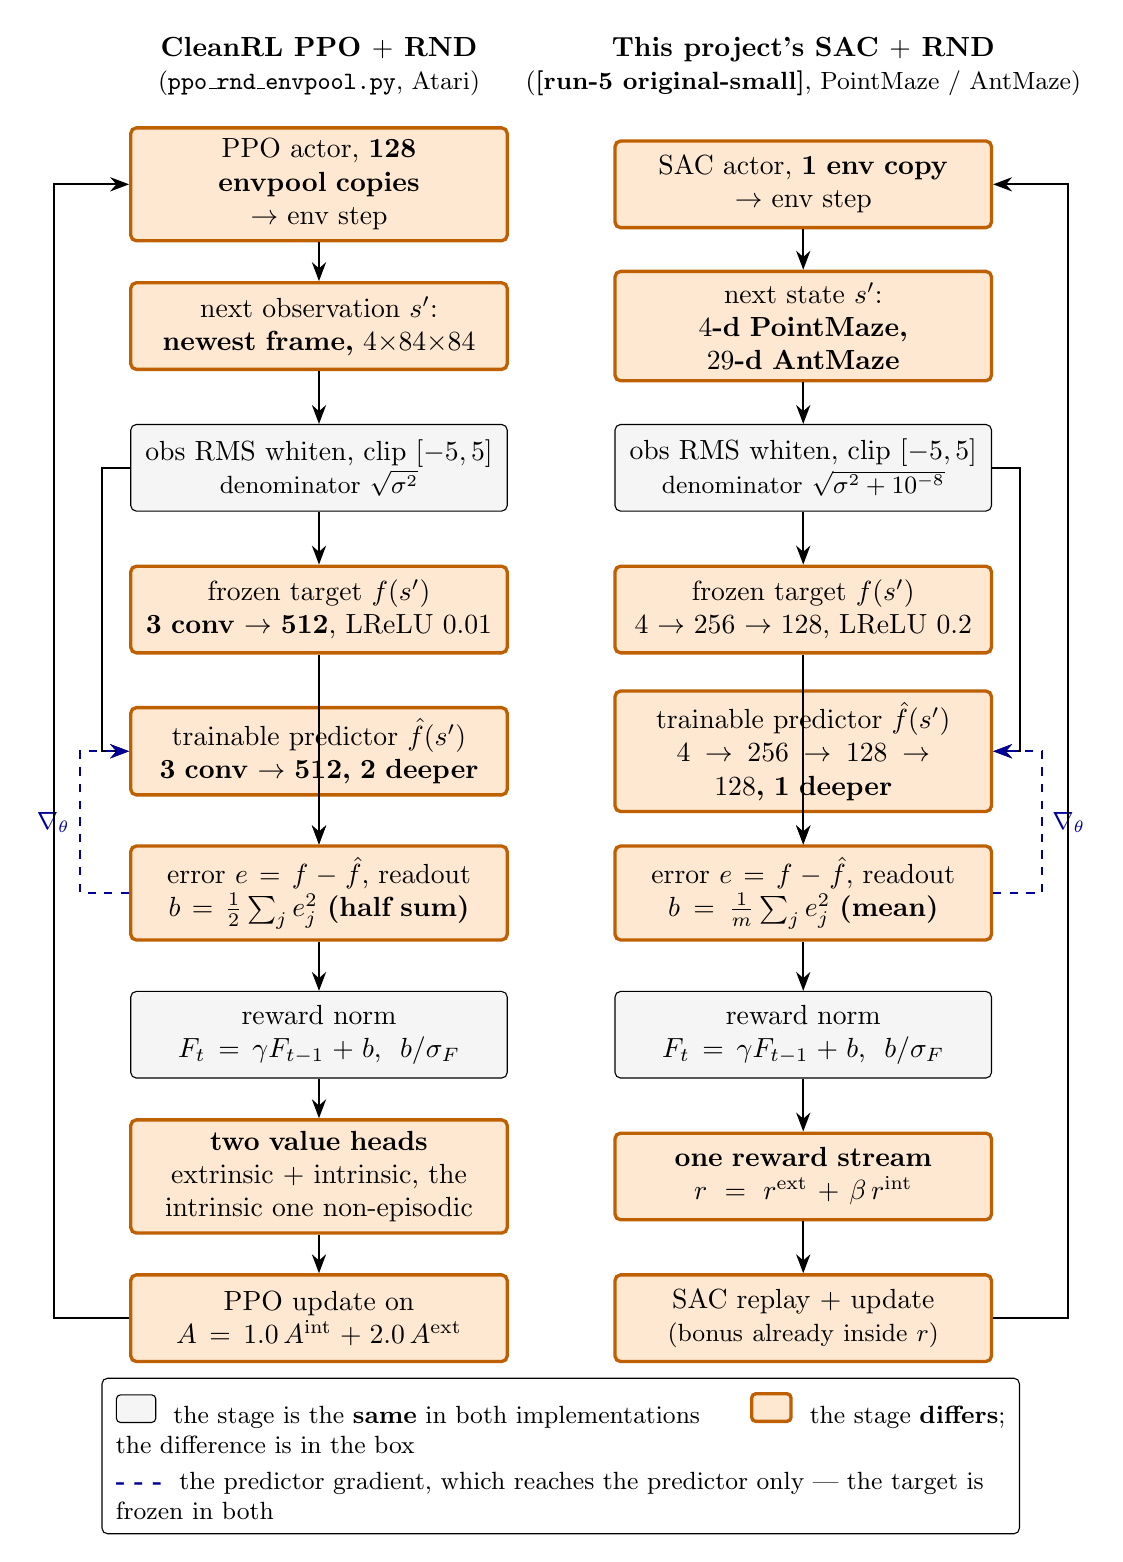
\begin{tikzpicture}[
  font=\normalsize,
  >={Stealth[length=2.4mm]},
  box/.style={draw,rounded corners=2pt,align=center,inner sep=4pt,
              minimum height=11mm,text width=45mm,fill=white},
  same/.style={box,fill=black!4},
  differs/.style={box,fill=orange!18,draw=orange!75!black,very thick},
  head/.style={align=center,font=\bfseries},
  flow/.style={->,thick},
  grad/.style={->,dashed,thick,blue!60!black},
  stat/.style={->,dotted,thick,orange!80!black},
]

% Column centres and row heights. Explicit coordinates keep the two columns row-aligned, which is
% the whole point of the figure.
\def\LX{0}
\def\RX{6.15}
\def\rowA{0}      \def\rowB{-1.80}  \def\rowC{-3.60}   \def\rowD{-5.40}
\def\rowE{-7.20}   \def\rowF{-9.00}  \def\rowG{-10.80}  \def\rowH{-12.60}
\def\rowI{-14.40}

% ---------------- column headings ----------------
\node[head] at (\LX,1.5) {CleanRL PPO $+$ RND\\{\normalfont\small(\texttt{ppo\_rnd\_envpool.py}, Atari)}};
\node[head] at (\RX,1.5) {This project's SAC $+$ RND\\{\normalfont\small(\textbf{[run-5 original-small]}, PointMaze / AntMaze)}};

% ---------------- left column: CleanRL ----------------
\node[differs] (L1) at (\LX,\rowA) {PPO actor, \textbf{128 envpool copies}\\$\to$ env step};
\node[differs] (L2) at (\LX,\rowB) {next observation $s'$:\\\textbf{newest frame, $4{\times}84{\times}84$}};
\node[same]    (L3) at (\LX,\rowC) {obs RMS whiten, clip $[-5,5]$\\{\small denominator $\sqrt{\sigma^2}$}};
\node[differs] (L4) at (\LX,\rowD) {frozen target $f(s')$\\\textbf{3 conv $\to$ 512}, LReLU $0.01$};
\node[differs] (L5) at (\LX,\rowE) {trainable predictor $\hat f(s')$\\\textbf{3 conv $\to$ 512, 2 deeper}};
\node[differs] (L6) at (\LX,\rowF) {error $e=f-\hat f$, readout\\$b=\tfrac12\sum_j e_j^2$ \textbf{(half sum)}};
\node[same]    (L7) at (\LX,\rowG) {reward norm\\$F_t=\gamma F_{t-1}+b$,\ \ $b/\sigma_F$};
\node[differs] (L8) at (\LX,\rowH) {\textbf{two value heads}\\extrinsic $+$ intrinsic, the\\intrinsic one non-episodic};
\node[differs] (L9) at (\LX,\rowI) {PPO update on\\$A=1.0\,A^{\mathrm{int}}+2.0\,A^{\mathrm{ext}}$};

% ---------------- right column: this project ----------------
\node[differs] (R1) at (\RX,\rowA) {SAC actor, \textbf{1 env copy}\\$\to$ env step};
\node[differs] (R2) at (\RX,\rowB) {next state $s'$:\\\textbf{$4$-d PointMaze, $29$-d AntMaze}};
\node[same]    (R3) at (\RX,\rowC) {obs RMS whiten, clip $[-5,5]$\\{\small denominator $\sqrt{\sigma^2+10^{-8}}$}};
\node[differs] (R4) at (\RX,\rowD) {frozen target $f(s')$\\\textbf{$4\to256\to128$}, LReLU $0.2$};
\node[differs] (R5) at (\RX,\rowE) {trainable predictor $\hat f(s')$\\\textbf{$4\to256\to128\to128$, 1 deeper}};
\node[differs] (R6) at (\RX,\rowF) {error $e=f-\hat f$, readout\\$b=\tfrac1m\sum_j e_j^2$ \textbf{(mean)}};
\node[same]    (R7) at (\RX,\rowG) {reward norm\\$F_t=\gamma F_{t-1}+b$,\ \ $b/\sigma_F$};
\node[differs] (R8) at (\RX,\rowH) {\textbf{one reward stream}\\$r=r^{\mathrm{ext}}+\beta\,r^{\mathrm{int}}$};
\node[differs] (R9) at (\RX,\rowI) {SAC replay $+$ update\\{\small(bonus already inside $r$)}};

% ---------------- forward edges, both columns ----------------
\foreach \a/\b in {L1/L2,L2/L3,L3/L4,L4/L6,L5/L6,L6/L7,L7/L8,L8/L9}{\draw[flow] (\a) -- (\b);}
\foreach \a/\b in {R1/R2,R2/R3,R3/R4,R4/R6,R5/R6,R6/R7,R7/R8,R8/R9}{\draw[flow] (\a) -- (\b);}
% The whitened observation feeds the predictor as well as the target; route it down the side so the
% predictor is fed from the same place the target is.
\draw[flow] (L3.west) -- ++(-0.36,0) |- (L5.west);
\draw[flow] (R3.east) -- ++(0.36,0) |- (R5.east);

% ---------------- predictor gradient, both columns ----------------
\draw[grad] (L6.west) -- ++(-0.62,0) |- node[pos=0.25,left,font=\small,blue!60!black]{$\nabla_\theta$} (L5.west);
\draw[grad] (R6.east) -- ++(0.62,0) |- node[pos=0.25,right,font=\small,blue!60!black]{$\nabla_\theta$} (R5.east);

% ---------------- the RL loop back to the actor ----------------
\draw[flow] (L9.west) -- ++(-0.95,0) |- (L1.west);
\draw[flow] (R9.east) -- ++(0.95,0) |- (R1.east);

% ---------------- legend ----------------
\node[draw,rounded corners=2pt,align=left,inner sep=5pt,font=\small,text width=113mm]
  at ($(\LX,\rowI)+(3.07,-1.75)$)
  {\tikz\node[draw,rounded corners=1.5pt,fill=black!4,minimum width=5mm,minimum height=3mm]{};\ \
   the stage is the \textbf{same} in both implementations \hfill
   \tikz\node[draw=orange!75!black,very thick,rounded corners=1.5pt,fill=orange!18,minimum width=5mm,minimum height=3mm]{};\ \
   the stage \textbf{differs}; the difference is in the box\\[2pt]
   \textcolor{blue!60!black}{\textbf{- - -}}\ \ the predictor gradient, which reaches the predictor only --- the target is frozen in both};

\end{tikzpicture}
\end{document}
